% +++++++++++++++++++++++++++++++++++++++++++++++++++++++++++++++++++++++++++++++++++++
% Linda 11/5/2015
% +++++++++++++++++++++++++++++++++++++++++++++++++++++++++++++++++++++++++++++++++++++

A complete list of effective operators with direct DM/boson couplings for
Dirac DM, up to dimension 7, can be found in~\cite{Cotta:2012nj, Carpenter:2012rg, Crivellin:2015wva}. 
Higher dimensional operators, up to dimension 8, leading to Higgs+MET signatures,
are mentioned in~\cite{Carpenter:2012rg, Berlin:2014cfa}. 

%%%%%%%%%%%Dimension 5 operators
\subsection{Dimension 5 operators}

The lowest dimension benchmark operators we may consider are effective dimension 5,
such as the one depicted in Figure~\ref{fig:modelMonoHEFT}.  

\begin{figure}[!htb]
	\centering
	\unitlength=0.005\textwidth
	\begin{feynmandiagram}[modelMonoHEFT]
		\fmfleft{i1,i2}
		\fmfright{o1,o2,ohidden,o3}
		\fmf{fermion}{i2,v1,i1}
		\fmflabel{\Large $q,g$}{i2}
		\fmflabel{\Large $\bar{q},g$}{i1}
		\fmf{dashes}{v1,v2}
		\fmfv{decor.shape=circle,decor.filled=shaded, decor.size=30,label={\Large $\text{EFT}(\lambda,,\Lambda)$},label.a=30,label.d=15}{v2}
		\fmf{dashes}{v2,o3}
		\fmflabel{\Large $h$}{o3}
		\fmf{fermion}{o2,v2,o1}
		\fmflabel{\Large ${\bar{\chi}}$}{o1}
		\fmflabel{\Large ${\chi}$}{o2}
		\fmfdot{v1}
	\end{feynmandiagram}
	\caption{Diagram for a dimension 5 operator giving rise to a Higgs+MET signature.}
	\label{fig:modelMonoHEFT}
\end{figure}

Following the notation of~\cite{Carpenter:2012rg},  models
from this category have a Lagrangian that includes terms such as:

\begin{eqnarray}
\frac{m_W^2}{\Lambda_5^3} ~\bar{\chi} \chi ~W^{+ \mu} W^{-}_\mu
+ \frac{m_Z^2}{2 \Lambda_5^3} ~ \bar{\chi} \chi ~ Z^\mu Z_\mu ~.
\end{eqnarray}

where $m_Z$ and $m_W$ are the masses of the $Z$ and $W$ boson, $W^{\mu}$ and $Z^{\mu}$
are the fields of the gauge bosons, $\chi$ denote the Dark Matter fields
and $\Lambda_5$ is the effective field theory scale. Note that these operators are of true dimension 7, 
but reduce to effective dimension 5 once Higgs vevs, contained in the W and Z mass terms, are inserted.  
As such, one expects  these that operators would naturally  arise in UV complete models where Dark Matter 
interacts via a Higgs portal where heavy mediators would couple to the Higgs or other fields in an extended Higgs sector. 
In such models the full theory may be expected to contain additional operators with Higgs-Dark Matter couplings. 

The Madgraph model parameters are:
xxhhg5, $\lambda$, $g_{DM} = \frac{(246 GeV)}{\lambda}$	

Concentrating  for the moment on mono-gauge boson signals, the above operator induces signatures with 
MET in conjunction with Z and W bosons at tree level,
while at loop level it induces couplings to photon pairs and $Z \gamma$ through W loops.
In these models, a clear relation exists between final states with photons, EW bosons
and Higgs boson. 

As shown in Fig.~\ref{fig:EW_EFT5_Zlep_MET}
kinematics of this model can be approximated by that of a simplified model including 
a high-mass scalar mediator exchanged in the s-channel. For this reason, 
the list of benchmark models with direct boson-DM couplings for photon, Z and W 
only includes dimension 7 operators: the scalar model with initial state radiation of an EW boson
is already recommended and its results can be rescaled. The Higgs+MET analysis
however will to use this model, as it would not be sensitive to a scalar mediator model. 

\begin{figure}
	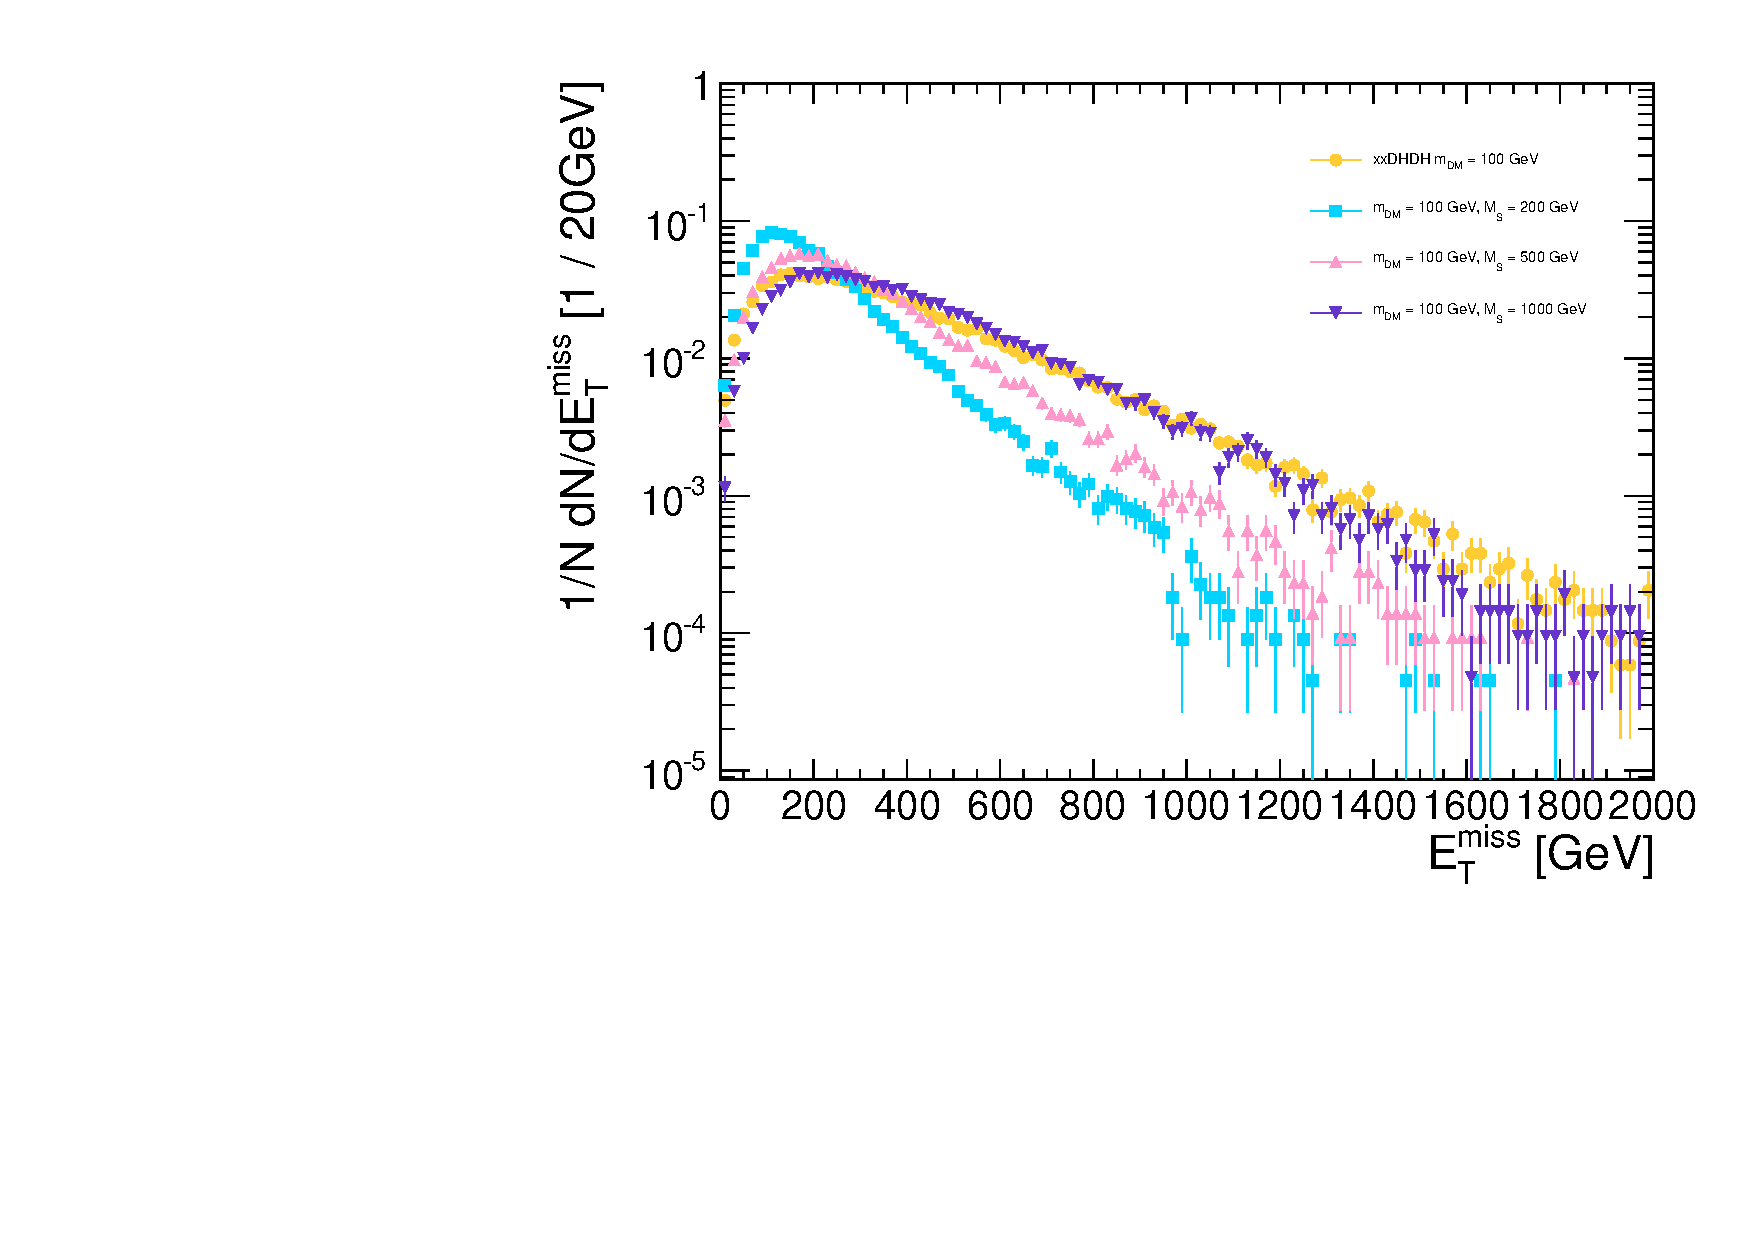
\includegraphics[width=0.6\textwidth]{figures/EW/pt_vv2_xxDHDH_vs_ScalarMediator.pdf}
	\caption{Comparison of the missing transverse momentum for the simplified model
		where a scalar mediator is exchanged in the s-channel and the model including 
		a dimension-5 scalar contact operator, in the leptonic Z+MET final state}
	\label{fig:EW_EFT5_Zlep_MET}
\end{figure}

\subsubsection{Parameter scan}

%\begin{figure}[!htbp]
%	\begin{minipage}{0.5\textwidth}
%		\centering
%		\includegraphics[width = \linewidth]{xxhhg5/truth_leading_b_pt.eps}
%	\end{minipage}
%	\begin{minipage}{0.5\textwidth}
%		\centering
%		\includegraphics[width = \linewidth]{xxhhg5/truth_leading_b_eta.eps}
%	\end{minipage}
%\end{figure}
%
%\begin{figure}[!htbp]
%	\begin{minipage}{0.5\textwidth}
%		\centering
%		\includegraphics[width = \linewidth]{xxhhg5/truth_subleading_b_pt.eps}
%	\end{minipage}
%	\begin{minipage}{0.5\textwidth}
%		\centering
%		\includegraphics[width = \linewidth]{xxhhg5/truth_subleading_b_eta.eps}
%	\end{minipage}
%\end{figure}
%
%\begin{figure}[!htbp]
%	\begin{minipage}{0.5\textwidth}
%		\centering
%		\includegraphics[width = \linewidth]{xxhhg5/truth_bb_deltar.eps}
%	\end{minipage}
%\end{figure}
%
%\FloatBarrier
%\clearpage


%%%%%%%%%%%%%Dimension 7 operators

\subsection{Dimension 7 operators}

% +++++++++++++++++++++++++++++++++++++++++++++++++++++++++++++++++++++++++++++++++++++
% Uli 3/5/2015
% +++++++++++++++++++++++++++++++++++++++++++++++++++++++++++++++++++++++++++++++++++++

The dimension-7 benchmark models  contain the $SU(2)_L \times U(1)_Y$ gauge-invariant couplings between 
DM fields and the kinetic terms of the EW bosons. The CP-conserving scalar couplings of this type can be written as
\begin{equation} \label{eq:Lc1c2}
\frac{c_1}{\Lambda_S^3} \, \bar \chi \chi \, B_{\mu \nu} B^{\mu \nu }  + \frac{c_2}{\Lambda_S^3} \, \bar \chi \chi \, W_{\mu \nu}^i W^{i, \mu \nu }  \,.
\end{equation}
Here $B_{\mu \nu} = \partial_\mu B_\nu - \partial_\nu B_\mu$ and $W_{\mu \nu}^i =  \partial_\mu W_\nu^i - \partial_\nu W_\mu^i + g_2 \hspace{0.25mm} \epsilon^{ijk}  \hspace{0.25mm}  W_\mu^j \hspace{0.25mm} W_\mu^k$ are the $U(1)_Y$ and $SU(2)_L$ field strength tensor, respectively, and  $g_2$ denotes the weak coupling constant. In the case of the pseudoscalar couplings, one has instead
\begin{equation} \label{eq:Lc3c4}
\frac{c_1}{\Lambda_P^3} \, \bar \chi \gamma_5 \chi \, B_{\mu \nu} \tilde B^{\mu \nu }  + \frac{c_2}{\Lambda_P^3} \, \bar \chi \gamma_5 \chi \, W_{\mu \nu}^i \tilde W^{i, \mu \nu }  \,,
\end{equation}
where $\tilde B_{\mu \nu} = 1/2 \hspace{0.5mm} \epsilon_{\mu \nu  \lambda \rho}  \hspace{0.25mm}  B^{\lambda \rho}$ and $\tilde W_{\mu \nu}^i = 1/2 \hspace{0.5mm} \epsilon_{\mu \nu  \lambda \rho}  \hspace{0.25mm}  W^{i, \lambda \rho}$ are the dual  field strength tensors. In addition to the CP-conserving interactions (\ref{eq:Lc1c2}) and (\ref{eq:Lc3c4}), there are also four CP-violating couplings that are obtained from the above operators by the replacement $\bar \chi \chi \leftrightarrow \bar \chi \gamma_5 \chi$.

The effective interactions introduced in (\ref{eq:Lc1c2}) and  (\ref{eq:Lc3c4}) appear  in models of Rayleigh DM~\cite{Weiner:2012cb}. Ultraviolet completions where the operators are generated through loops of states charged under $U(1)_Y$ and/or $SU(2)_L$  have been proposed in \cite{Weiner:2012gm} and their LHC signatures have been studied in \cite{Liu:2013gba}. If these new charged particles  are  light, the high-$p_T$ gauge bosons that participate in  the MET processes considered here are able to resolve the substructure of the loops. This generically suppresses the cross sections compared to the EFT predictions~\cite{Haisch:2012kf}, and thus will weaken the bounds on the interaction strengths of  DM and the EW gauge bosons  to some extent.  Furthermore, the light charged mediators may be produced  on-shell in $pp$ collisions, rendering direct LHC searches potentially more restrictive than MET searches. Making the above statements precise would require further studies beyond the timescale of this forum.

Since for $\Lambda_S = \Lambda_P$ the effective interactions (\ref{eq:Lc1c2}) and (\ref{eq:Lc3c4}) predict essentially the same value of the mono-photon, mono-$Z$ and mono-$W$ cross section \cite{Carpenter:2012rg,Crivellin:2015wva}, we consider below only the former couplings. We emphasise however that measurements of the jet-jet azimuthal angle difference in  MET$+ 2 j$ events may be used to disentangle whether DM couples more strongly to the combination $B_{\mu \nu} B^{\mu \nu}$ ($W_{\mu \nu}^i W^{i, \mu \nu }$) or the product $B_{\mu \nu} \tilde B^{\mu \nu}$ ($W_{\mu \nu}^i \tilde W^{i, \mu \nu }$) of field strength tensors \cite{Cotta:2012nj,Crivellin:2015wva}.

After EW symmetry breaking the interactions (\ref{eq:Lc1c2}) induce direct couplings between pairs of DM particles and  gauge bosons.  The corresponding Feynman rule reads
\begin{equation}  \label{eq:feynman}
\frac{4 \hspace{0.25mm} i}{\Lambda_S^3} \; g_{V_1 V_2} \, \big (  p_1^{\mu_2} \hspace{0.25mm} p_2^{\mu_1} - g^{\mu_1 \mu_2}  \, p_1 \cdot p_2 \big ) \,,
\end{equation}
where $p_i$ ($\mu_i$) denotes the momentum (Lorentz index) of the vector field $V_i$ and for simplicity the spinors associated with the DM fields have been dropped. The couplings $g_{V_i V_j}$ take the form
\begin{equation} \label{eq:gViVj}
\begin{split}
g_{\gamma \gamma} & = c_w^2 \hspace{0.25mm} c_1+ s_w^2  \hspace{0.25mm} c_2 \,, \\[1mm]
g_{\gamma Z}   & = - s_w c_w \, \big (  c_1  - c_2  \big ) \,, \\[1mm]
g_{ZZ}  & = s_w^2 \hspace{0.25mm} c_1 + c_w^2  \hspace{0.25mm} c_2  \,, \\[1mm]
g_{WW} & = c_2 \,,
\end{split}
\end{equation}
with $s_w$ ($c_w$) the sine (cosine) of the weak mixing angle. Note that our coefficients $c_1$ and $c_2$ are identical to the coefficients $C_B$ and $C_W$ used in \cite{Crivellin:2015wva}, while they are related via $k_1 = \frac{1}{{c_w}^2} c_1$ and $k_2 = \frac{1}{{s_w}^2} c_2$ to the coefficients $k_1$ and $k_2$ introduced in \cite{Carpenter:2012rg}.

The coefficients $c_1$ and $c_2$ appearing in (\ref{eq:gViVj}) determine the relative importance of each of the MET channels and their correlations. For example, one observes that:
\begin{itemize}
 \item Only $c_2$ enters the coupling between DM and $W$ bosons, meaning that only models with $c_2 \neq 0$ predict a mono-$W$ signal;
 \item If $c_1 = c_2$ the mono-photon (mono-$Z$) signal does not receive contributions from diagrams involving $Z$ (photon) exchange;
  \item Since numerically $c_w^2/s_w^2 \simeq 3.3$ the mono-photon channel is particularly sensitive to $c_1$.
\end{itemize}


% +++++++++++++++++++++++++++++++++++++++++++++++++++++++++++++++++++++++++++++++++++++
% +++++++++++++++++++++++++++++++++++++++++++++++++++++++++++++++++++++++++++++++++++++

The kinematic distributions for dimension-7 scalar and pseudoscalar operators
only shows small differences, as shown in Fig.~\ref{fig:EW_EFT5_gamma_MET}.

\begin{figure}
    
\includegraphics[width=0.6\textwidth]{figures/llug}
    \caption{Comparison of the missing transverse momentum for the scalar and pseudoscalar
    operators with direct interaction between DM and photon, in the photon+MET final state}
    \label{fig:EW_EFT5_gamma_MET}
\end{figure}

Similarly, the differences in kinematics for the various signatures
are negligible when changing the coefficients $k_1$ and $k_2$, as shown
in Figure~\ref{EFTD7_EW_kinematics}. Only the case $k_1=k_2=1$ is generated as benchmark;
other cases are left for reinterpretation as they will only need a rescaling of the cross-sections
shown in Appendix~\ref{app:EWSpecificModels_Appendix} for the various DM
mass points considered.

\begin{figure}[h!]
  \centering
  \subfloat[Missing transverse momentum distribution for the photon+MET final state.\label{fig:EFTD7_EW_gamma_MET}]{%
      
\includegraphics[width=0.45\textwidth]{figures/gull}
    }
    \hfill
  \subfloat[Missing transverse momentum distribution for the leptonic Z+MET final state.\label{fig:EFTD7_EW_Z_MET}]{%
      
\includegraphics[width=0.45\textwidth]{figures/llug}
    }
  \subfloat[Transverse mass ($m_T$) for the leptonic W+MET final state.\label{fig:EFTD7_EW_Wlep_mT}]{%
      
\includegraphics[width=0.45\textwidth]{figures/gull}
    }
    \caption{Kinematic distributions relevant for searches with W, Z and photons in the final state,
    for for the scalar and pseudoscalar operators representing direct interactions between DM and bosons.}
    \label{fig:EFTD7_EW_kinematics}

\end{figure}

Examples of relevant kinematic distributions for selected benchmark points are
shown in Fig.~\ref{fig:DMV_EW_kinematics}.

\begin{figure}[h!]
  \centering
  \subfloat[Missing transverse momentum distribution for the photon+MET final state.\label{fig:DMV_EW_gamma_MET}]{%
      
\includegraphics[width=0.45\textwidth]{figures/gull}
    }
    \hfill
  \subfloat[Missing transverse momentum distribution for the leptonic Z+MET final state.\label{fig:DMV_EW_Z_MET}]{%
      
\includegraphics[width=0.45\textwidth]{figures/llug}
    }
  \subfloat[Transverse mass ($m_T$) for the leptonic W+MET final state.\label{fig:DMV_EW_Wlep_mT}]{%
      
\includegraphics[width=0.45\textwidth]{figures/gull}
    }
    \hfill
  \subfloat[Fat \textbf{[Insert algorithm]} jet mass ($m_T$) for the the hadronic W+MET final state.\label{fig:DMV_EW_Whad_jetMass}]{%
      
\includegraphics[width=0.45\textwidth]{figures/llug}
    }
    \caption{Kinematic distributions relevant for searches with W, Z and photons in the final state,
    for the simplified model with a vector mediator exchanged in the $s-$channel.}
    \label{fig:DMV_EW_kinematics}
\end{figure}

%%%%%%%%%%%%%Dimension 8 operators

\subsection{Higher dimensional operators}

Higher dimensional operators (dimension 8) have the form 

$$\bar{\chi} \gamma^{\mu} \chi B_{\mu \nu} H^{\dagger} D^{\nu} H$$

The Madgraph parameters are:
xgxFhDh, $\Lambda$, $y_{\chi} = \frac{1}{\Lambda^{4}}$	

%\subsection{xgxFhDh Truth Kinematics}
%
%\begin{figure}[!htbp]
%	\begin{minipage}{0.5\textwidth}
%		\centering
%		\includegraphics[width = \linewidth]{xgxFhDh/truth_leading_b_pt.eps}
%	\end{minipage}
%	\begin{minipage}{0.5\textwidth}
%		\centering
%		\includegraphics[width = \linewidth]{xgxFhDh/truth_leading_b_eta.eps}
%	\end{minipage}
%\end{figure}
%
%\begin{figure}[!htbp]
%	\begin{minipage}{0.5\textwidth}
%		\centering
%		\includegraphics[width = \linewidth]{xgxFhDh/truth_subleading_b_pt.eps}
%	\end{minipage}
%	\begin{minipage}{0.5\textwidth}
%		\centering
%		\includegraphics[width = \linewidth]{xgxFhDh/truth_subleading_b_eta.eps}
%	\end{minipage}
%\end{figure}
%
%\begin{figure}[!htbp]
%	\begin{minipage}{0.5\textwidth}
%		\centering
%		\includegraphics[width = \linewidth]{xgxFhDh/truth_bb_deltar.eps}
%	\end{minipage}
%\end{figure}
%
%\FloatBarrier
%\clearpage


\subsection{Completion and validity of EW contact operators}

\textbf{[TODO: mention here discussion with Liantao yesterday]}

% +++++++++++++++++++++++++++++++++++++++++++++++++++++++++++++++++++++++++++++++++++++
%   Linda 11/5/15
% +++++++++++++++++++++++++++++++++++++++++++++++++++++++++++++++++++++++++++++++++++++

As an example of a simplified model corresponding to the dimension-5 EFT operator 
described above, we consider a Higgs portal with a scalar mediator. Models of this kind
are among the most concise versions of simplified models that produce 
couplings of Dark Matter to pairs of gauge-bosons.  Scalar fields may couple directly to pairs of electroweak gauge bosons, 
but must carry part of the electroweak vev.  One may thus consider a simple model where Dark Matter couples to a a scalar 
singlet mediator, which mixes with the fields in the Higgs sector.
\begin{equation}
L\subset m_s S^2 + \lambda S^2H^2 +\lambda^{'} S H^2 + y S \chi \overline{\chi}
\end{equation}
Where H is a field in the Higgs sector that contains part of the electroweak vev, 
S is a heavy scalar singlet and $\chi$ is a Dark Matter field. 
There is then an S channel diagram where DM pairs couple to the singlet field S, 
which then mixes with a Higgs-sector field, and couples to W and Z bosons. 
This diagram contains 2 insertions of EW symmetry breaking fields, 
corresponding in form to the effective dimension-5 operator in the previous section.   

\subsection{Model implementation}

These models are generated at leading
order with MadGraph 2.2.2, using Pythia8 for the parton shower.
Parameter cards can be found on the Forum SVN repository:~\cite{ForumSVN_EWEFTD7} for dimension 5 operators
and ~\cite{ForumSVN_EWEFTD7} for dimension 7.
